\subsection{$\nox$ sensor cross-sensitivity}
Commercial $\nox$ sensors are cross-sensitive to tailpipe ammonia. Figure~\ref{fig::cross_sensitivity} shows the effect of cross-sensitivity on commercial $\nox$ sensors due to tailpipe ammonia. When the tailpipe ammonia is greater than a threshold value, the $\nox$ sensor output is corrupted, as shown in the plots where the $\nox$ sensor measurement is significantly higher than the FTIR measurement, which can be considered the true value. The resulting
error is modeled as a function of ammonia concentration and a temperature-dependent cross-sensitivity factor $\chi(T)$.
This introduces a non-negative directional error $\lr{\varepsilon_\chi= \chi\lr{T(k)} \times \con{\ammonia}^{out}\geq 0}$
into the tailpipe $\nox$ measurement $y_1$. Accordingly, when the $\nox$ reduction in a time step is calculated from
sensor measurements, $y_1(k) = x_1(k) + \varepsilon_{\chi}(k)$, the estimated quantity is less than the actual $\nox$
reduction:
\begin{align}
        \eta_y(k) &= u_1(k-1) - y_1(k) =  \eta(k) - \varepsilon_\chi(k) \leq \eta(k) \label{eqn::cross_meas}
\end{align}
Thus, the bounding condition on the saturated system's response (\ref{eqn::eta_bound}) remains valid when the $\nox$ reduction during the time step is estimated from the $\nox$ sensor measurements:
\begin{align}
        \eta_{sat}(k) &\geq \eta(k) = \eta_y(k) + \varepsilon_\chi(k) \geq \eta_y(k) \label{eqn::eta_y_bound}
\end{align}
%===
\begin{figure}[ht]
        \centering
        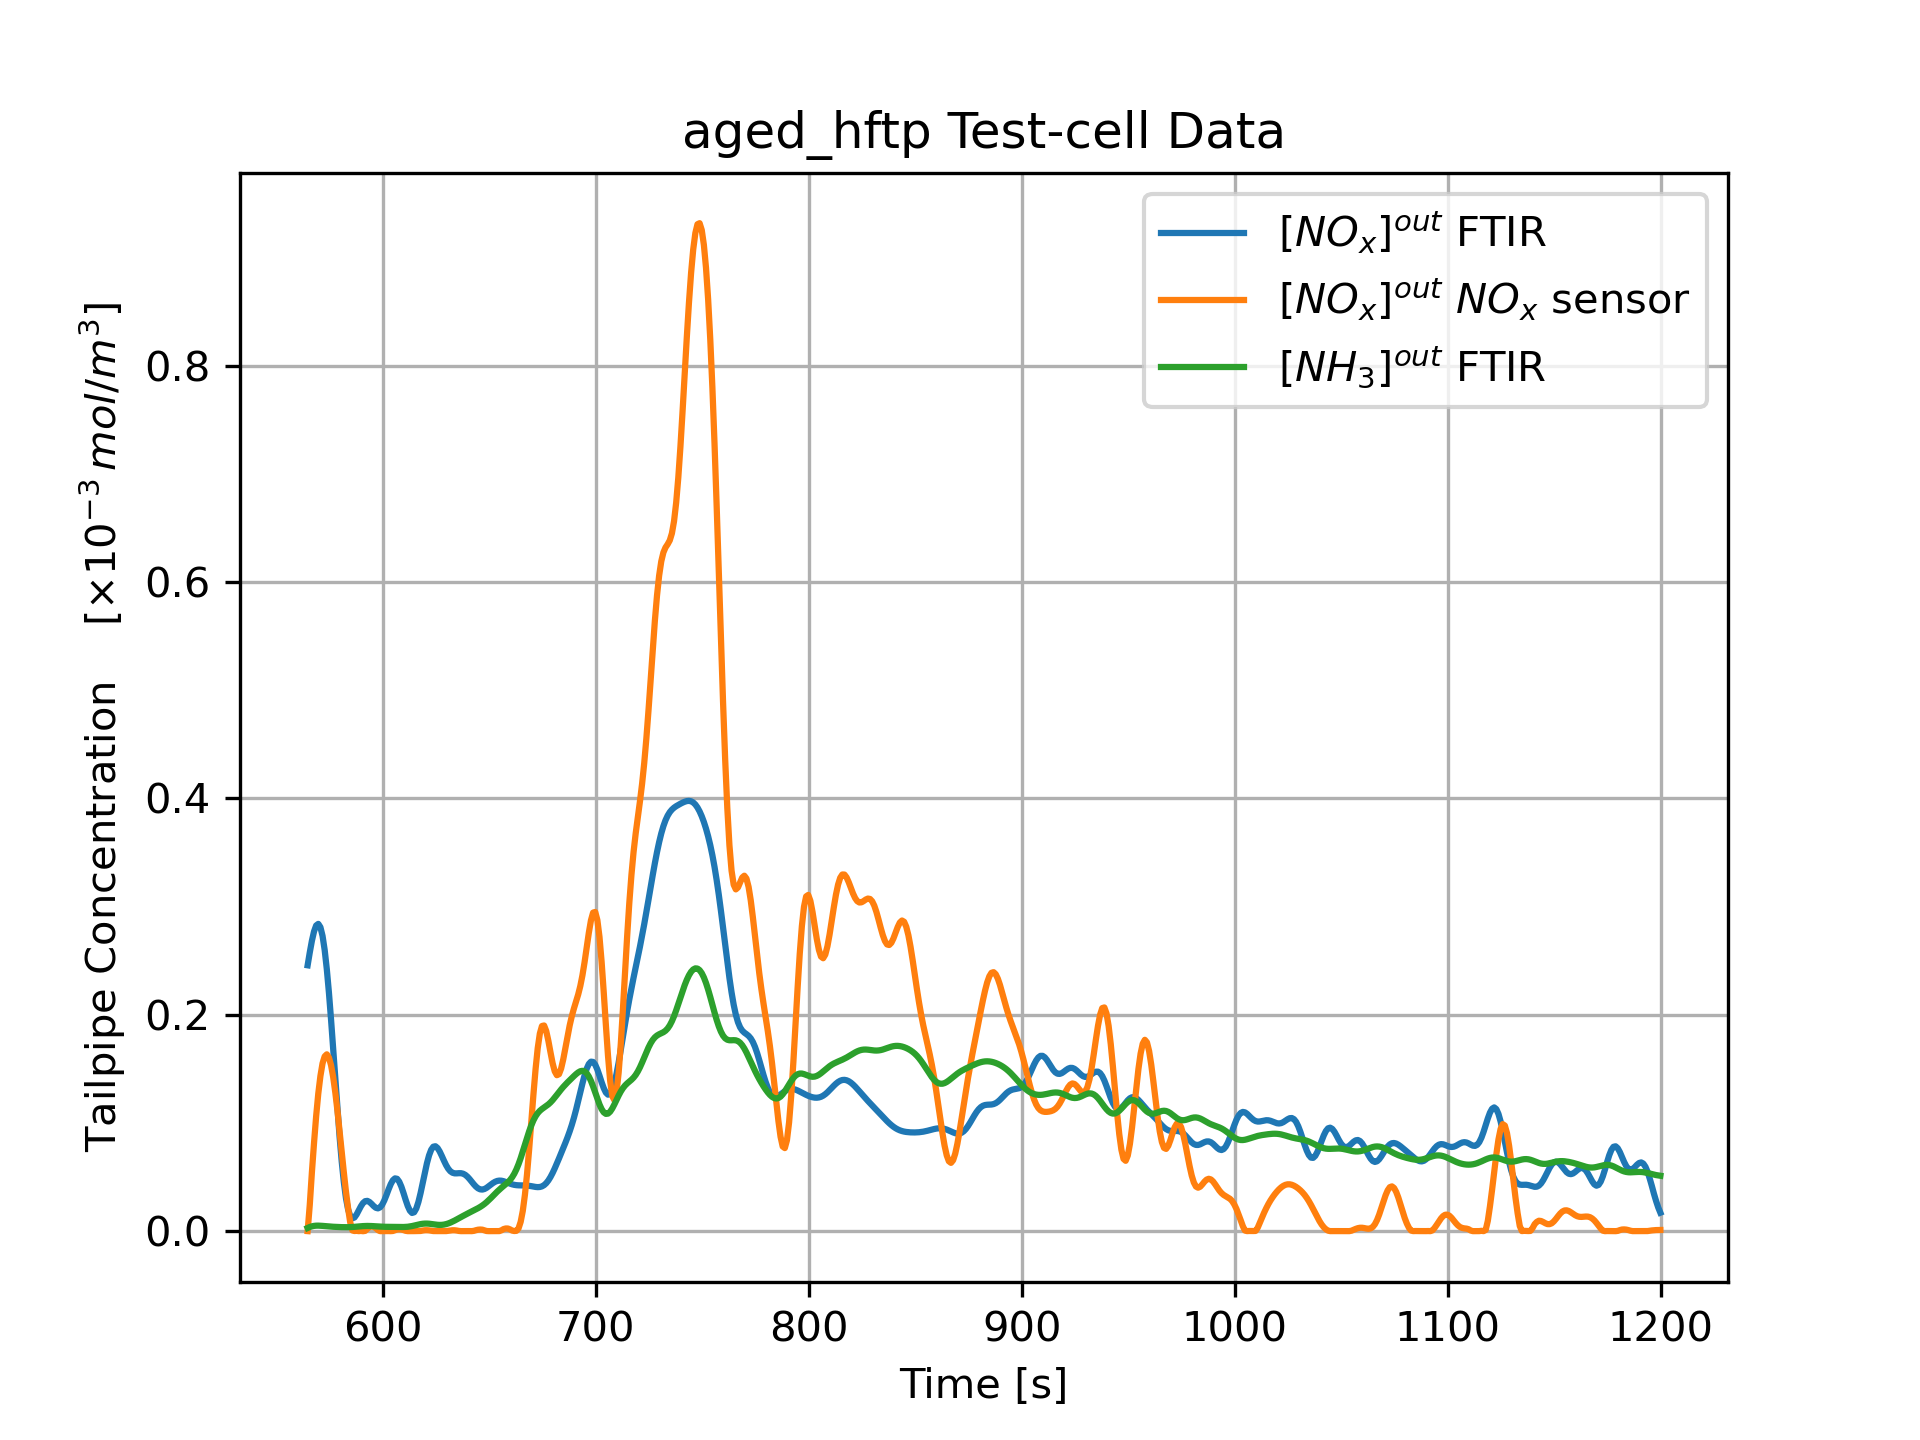
\includegraphics[width=\figWidth]{./figs/2_mdl/cross_aged_hftp.png}
        \caption{$\nox$ sensor cross-sensitivity to tailpipe ammonia}
        \label{fig::cross_sensitivity}
\end{figure}
% The FTIR sensor also has a bias that is directional. Similar arguments as above can be made for the validity of the
% bounding condition.
